\documentclass[brazil,pagestart=firstchapter]{abnt}

% This does not accept all Unicode chars (for instance: I²C gives an error)
%\usepackage[utf8]{inputenc}

% This adds support for Unicode chars.
\usepackage{ucs}
\usepackage[utf8x]{inputenc}

\usepackage[brazil]{babel}

% http://tex.stackexchange.com/questions/664/why-should-i-use-usepackaget1fontenc
% http://texblog.net/latex-archive/fonts/symbols/
\usepackage[T1]{fontenc}

% Use another font:
% http://tex.stackexchange.com/questions/553/what-packages-do-people-load-by-default-in-latex/951#951
%\usepackage{lmodern}

% 'microtype' improves LaTeX line-breaking algorithm by using
% microtypographic features of the font
% http://tex.stackexchange.com/questions/349/what-is-the-practical-difference-between-latex-and-pdflatex/358#358
\usepackage{microtype}


%%%%%%%%%%%%%%%%%%%%%%%%%%%%%%%%%%%%%%%%%%%%%%%%%%%%%%%%%%%%
% Acronyms and abbreviations

% Simple and effective acronym package:
\usepackage[printonlyused,withpage]{acronym}

% This one from abntex does not work correctly:
% http://comments.gmane.org/gmane.comp.tex.brazilian/13365
%\usepackage{tabela-simbolos}

% "nomencl" is quite annoying to use, specially when compared to "acronym".
% "nomencl" requires an external file and some extra commands.
% "acronym", on the other hand, just works out of the box!
%\usepackage{nomencl}
%\makenomenclature
% http://en.wikibooks.org/wiki/LaTeX/Indexing#Abbreviation_list
% http://franz.kollmann.in/latex/latex.html#abbr
% latexmk needs a custom dependency for this package
% http://magic.aladdin.cs.cmu.edu/2007/11/06/continuous-latex-compilation-using-latexmk/


%%%%%%%%%%%%%%%%%%%%%%%%%%%%%%%%%%%%%%%%%%%%%%%%%%%%%%%%%%%%
% Other packages

% Adding \textsubscript{}
% LaTeX already has \textsuperscript, but lacks \textsubscript.
% http://en.wikibooks.org/wiki/LaTeX/Formatting#Text_mode_superscript_and_subscript
\usepackage{fixltx2e}

% Better handling of space after a custom command.
% http://tex.stackexchange.com/questions/17730/newcommand-and-spacing
\usepackage{xspace}

% Required for including graphics
\usepackage{graphicx}

% SI Units
% https://bitbucket.org/josephwright/siunitx/issue/100/undefined-control-sequence-bit-and-byte
\usepackage{siunitx}
\sisetup{
	load-configurations = binary,
	per-mode = symbol,
	list-final-separator = { e },
	range-phrase = { a },
	output-decimal-marker = {,}
}

% To find the total number of pages
%\usepackage{lastpage}

%%%%%%%%%%%%%%%%%%%%%%%%%%%%%%%%%%%%%%%%%%%%%%%%%%%%%%%%%%%%
% Embedding source-code

% For inserting source-code
%\usepackage{listings}
% TODO: configure this

% Settings I had from another project:
%% Setting the default listings font size
%\lstset{
%	basicstyle=\ttfamily\footnotesize
%}
%
%% AVISO!!!
%% Dentro dos exemplos de código-fonte abaixo, coloquei um "tab" de
%% indentação por estar dentro de um "frame", e "espaços" para a
%% indentação do código de exemplo. Isto foi necessário porque os tabs
%% estavam sendo ignorados dentro do códigos de exemplo.
%
%\lstnewenvironment{shellcode}[1][]
%{\lstset{language=bash,
%	basicstyle=\ttfamily\footnotesize,
%	escapeinside={(*@}{@*)},
%	breaklines=true,
%	breakatwhitespace=true,
%	showspaces=false,
%	showstringspaces=false,
%	frame=shadowbox,
%	rulecolor=\color{black},
%	rulesepcolor=\color{black},
%	#1}
%}{}
%
%\lstnewenvironment{pythoncode}[1][]
%{\lstset{language=Python,
%	basicstyle=\ttfamily\footnotesize,
%	escapeinside={(*@}{@*)},
%	%numbers=left,
%	breaklines=true,
%	breakatwhitespace=true,
%	showspaces=false,
%	showstringspaces=false,
%	frame=shadowbox,
%	frameround=rrrt,
%	rulecolor=\color{black},
%	rulesepcolor=\color{gray},
%	#1}
%}{}


%%%%%%%%%%%%%%%%%%%%%%%%%%%%%%%%%%%%%%%%%%%%%%%%%%%%%%%%%%%%
% Table-related packages:

% For multirow cells inside tabular environments
%\usepackage{multirow}

% Longtable allows you to write tables that continue to the next page
%\usepackage{longtable}

% 'tabularx' package - simple column stretching
% http://en.wikibooks.org/wiki/LaTeX/Tables#The_tabularx_package_-_simple_column_stretching
%\usepackage{tabularx}

% 'booktabs' - Publication quality tables in LaTeX
%\usepackage{booktabs}

% Alternating row colors in tables
%\usepackage[table]{xcolor}
%\definecolor{tabular-odd-color}{gray}{0.90}
%\definecolor{tabular-even-color}{gray}{0.97}


%%%%%%%%%%%%%%%%%%%%%%%%%%%%%%%%%%%%%%%%%%%%%%%%%%%%%%%%%%%%
% Fancy headers (and footers)
% http://en.wikibooks.org/wiki/LaTeX/Page_Layout#Page_Styles
%\usepackage{fancyhdr}
%\pagestyle{fancy}
%
%% Headers and footers definition:
%\lhead{\includegraphics[height=21mm]{shared/2aliancas_h.pdf}}
%\chead{}
%% This \parbox is a hack to keep text aligned at top, but it's not the
%% only available solution:
%% http://tex.stackexchange.com/questions/2440/how-to-vertically-align-headers-footers-in-fancyhdr-package
%\rhead{\parbox[b][21mm][t]{0.65\textwidth}{\raggedleft\large\titletext \\[1em] \subtitletext}}
%\lfoot{}
%\cfoot{}
%\rfoot{Page \thepage{} of \pageref{LastPage}}
%
%\renewcommand{\headrulewidth}{0pt}  % Default is 0.4pt
%\renewcommand{\footrulewidth}{0pt}  % Default is 0pt


%%%%%%%%%%%%%%%%%%%%%%%%%%%%%%%%%%%%%%%%%%%%%%%%%%%%%%%%%%%%
% 'hyperref' for including hyperlinks to the PDF.
% It should be loaded last.
% http://en.wikibooks.org/wiki/LaTeX/Formatting#Typesetting_URLs
\usepackage{hyperref}
\hypersetup{
	pdfborder={0 0 0},
	hyperindex=false
}
% hyperindex=false is required by "tabela-de-simbolos"

% http://en.wikibooks.org/wiki/LaTeX/Labels_and_Cross-referencing#Issues_with_links_to_tables_and_figures_handled_by_hyperref
%\usepackage[all]{hypcap}


%%%%%%%%%%%%%%%%%%%%%%%%%%%%%%%%%%%%%%%%%%%%%%%%%%%%%%%%%%%%
% Custom commands

\newcommand{\VBUS}{V\textsubscript{BUS}\xspace}
\newcommand{\VCC}{V\textsubscript{CC}\xspace}
\newcommand{\GND}{GND\xspace}

%%%%%%%%%%%%%%%%%%%%%%%%%%%%%%%%%%%%%%%%%%%%%%%%%%%%%%%%%%%%
% Some metadata

% This is used only by latex-beamer package:
%\title{Mouse USB usando magnetômetro}
%\author{Denilson Figueiredo de Sá}
%\date{2011-11-16}
%\institute{DCC/UFRJ}
%\keywords{AVR, USB, mouse, magnetometer}

\autor{Denilson Figueiredo de Sá}
\titulo{Mouse USB usando magnetômetro}
\orientador{Nelson Quilula Vasconcelos}
%\comentario{}
\instituicao{Departamento de Ciência da Computação \par Instituto de Matemática \par Universidade Federal do Rio de Janeiro}
\local{Rio de Janeiro - RJ, Brasil}
\data{16 de novembro de 2011}

% latex-beamer sets the pdftitle and pdfauthor automatically, but here we
% must explicitly run it:
\hypersetup{
	pdftitle={\ABNTtitulodata},
	pdfauthor={\ABNTautordata}
}

%%%%%%%%%%%%%%%%%%%%%%%%%%%%%%%%%%%%%%%%%%%%%%%%%%%%%%%%%%%%
\begin{document}

% The "abnt" class issues a warning:
%   pdfTeX warning (ext4): destination with the same identifier
%   (name{page.i}) has been already used, duplicate ignored
% This page has a solution (or workaround):
% http://en.wikibooks.org/wiki/LaTeX/Hyperlinks#Problems_with_Links_and_Pages
%\pagenumbering{roman}
% But, anyway, it's better to ignore that warning (or even better would be
% to report it to abntex maintainers).
% Instead of messing with page numbering, I've added pagestart=firstchapter
% option.


\capa

\folhaderosto


\begin{folhadeaprovacao}

\setlength{\ABNTsignthickness}{0.4pt}
\setlength{\ABNTsignskip}{2cm}
\hspace*{1cm}

\centerline{\textbf{\large \ABNTtitulodata}}

\bigskip
\bigskip

\centerline{\textbf{\ABNTautordata}}

\bigskip
\bigskip

Projeto Final de Curso submetido ao Departamento de Ciência da Computação
do Instituto de Matemática da Universidade Federal do Rio de Janeiro como
parte dos requisitos necessários para obtenção do grau de Bacharel em
Ciência da Computação.

Apresentado por:

\assinatura{\ABNTautordata}

Aprovado por:

\assinatura{Prof. Nelson Quilula Vasconcelos \\ Orientador}
\assinatura{Prof. Adriano Joaquim}
\assinatura{Profª. Silvana Rossetto}

\bigskip
\bigskip
\bigskip

\begin{center}
\ABNTlocaldata

\ABNTdatadata
\end{center}

\end{folhadeaprovacao}


% Colocar o Sumário aqui é muito bom, mas não é de acordo com a norma ABNT
% NBR 14724: informação e documentação: trabalhos acadêmicos: apresentação.
%\tableofcontents{}


%\pretextualchapter{Dedicatória}
% TODO: escrever dedicatória (opcional)

%\pretextualchapter{Agradecimentos}
% TODO: escrever agradecimentos


\begin{resumo}
O resumo será escrito aqui.
\end{resumo}

\begin{abstract}
This will be the abstract, someday.
\end{abstract}


\listoffigures

%\listoftables


% The following command does not work:
% \listadesiglas
% Instead, I'm using "acronym" package.

\pretextualchapter{Lista de Siglas}

\begin{acronym}[EEPROM]

\acro{USB}{Universal Serial Bus}
\acro{HID}{Human Interface Device}

\acro{NRZI}{Non-Return-to-Zero Inverted}
\acro{SE0}{Single-ended 0}
\acro{SE1}{Single-ended 1}

\acro{I2C}[I²C]{Inter-Integrated Circuit}
\acro{TWI}{Two-Wire Interface}

\acro{ISP}{In-System Programmer}
\acro{ICSP}{In-Circuit Serial Programmer}

\acro{SRAM}{Static Random-Access Memory}
\acro{ROM}{Read-Only Memory}
\acro{EEPROM}{Electrically Erasable Programmable Read-Only Memory}

\end{acronym}


\tableofcontents


\chapter{Introdução\label{cap:introducao}}

Falar sobre: motivação, resumo, possíveis aplicações (palestras,
necessidades especiais, interatividade em jogos e exposições)

\section{Trabalhos relacionados\label{sec:trabalhos_relacionados}}

TrackIR, Wiimote, eye-tracking


\chapter{Protocolos e componentes\label{cap:protocolos_e_componentes}}

\section{USB\label{sec:usb}}

\ac{USB} é um protocolo que foi desenvolvido a partir do ano de 1994 pelas
empresas \textit{Compaq}, \textit{Hewlett-Packard}, \textit{Intel},
\textit{Lucent}, \textit{Microsoft}, \textit{NEC} e \textit{Philips}. Foi
motivado pela inexistência de um barramento bidirecional de baixo custo para
periféricos de baixa e média velocidade, assim como a falta de flexibilidade
dos barramentos até então existentes, os quais eram projetados para usos
bastante específicos, sendo impossível reutilizá-los para outros
periféricos. \cite{usb20}

A primeira versão do \ac{USB}, conhecida como ``USB 1.0'', foi oficialmente
lançada em janeiro de 1996 e definiu duas velocidades: \textit{low speed}
(\SI{1.5}{\mega\bit\per\second}) e \textit{full speed}
(\SI{12}{\mega\bit\per\second}). Alguns anos depois, em setembro de 1998, foi
lançada sua primeira revisão, ``USB 1.1'', que resolveu alguns problemas da
versão anterior mas não introduziu nenhuma mudança significativa.

A primeira grande revisão do protocolo foi lançada em abril de 2000, com o
nome de ``USB 2.0''. Esta versão introduziu uma terceira velocidade --
\textit{high speed} (\SI{480}{\mega\bit\per\second}) -- mas manteve total
compatibilidade com a revisão anterior do protocolo: dispositivos USB 1.x
funcionam em \textit{hosts} USB 2.0, e dispositivos USB 2.0 funcionam em
\textit{hosts} USB 1.x (porém limitados a \textit{full speed}).

\begin{figure}[h]
\centering
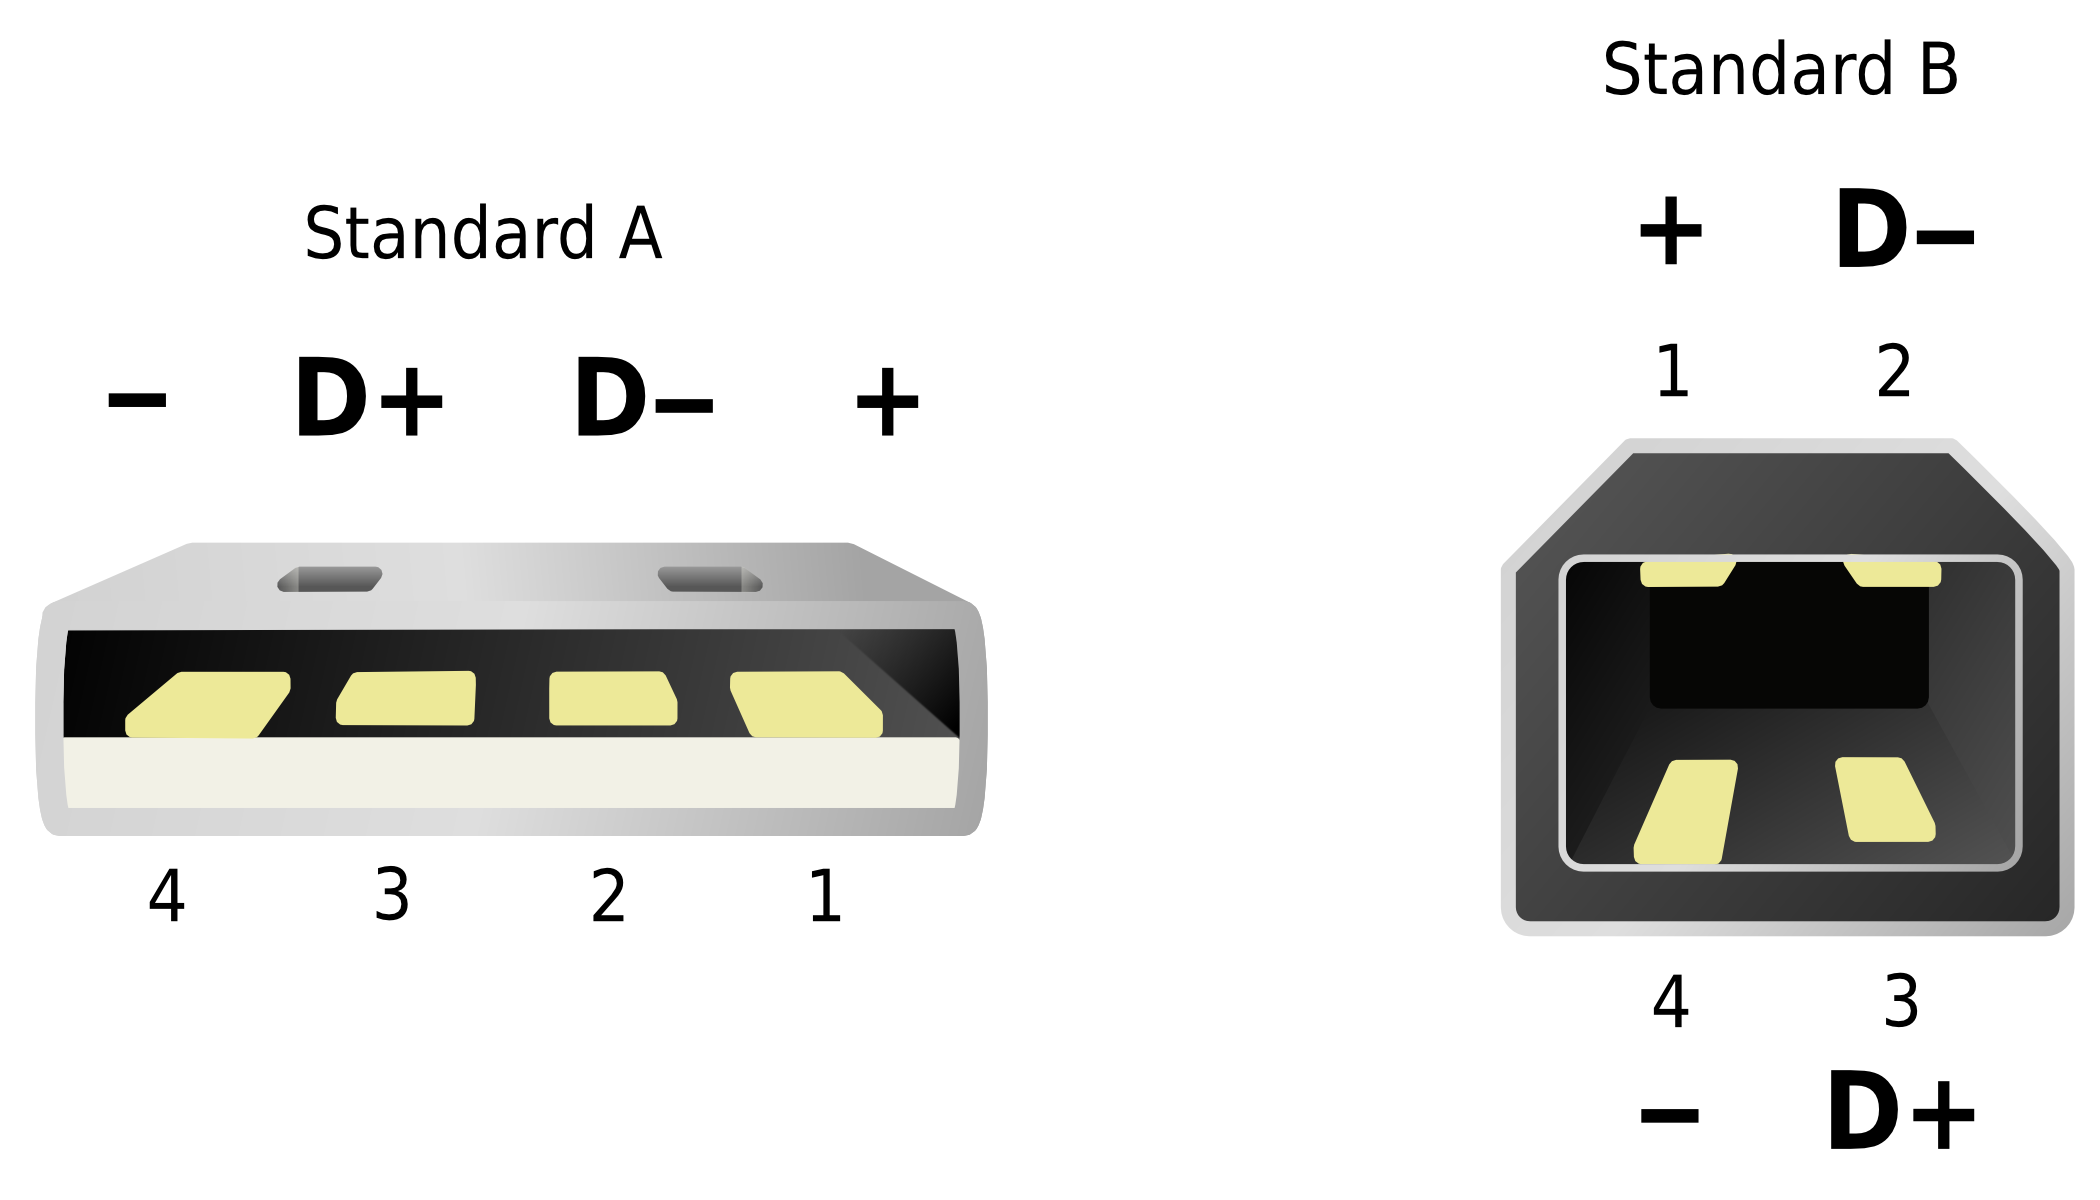
\includegraphics[width=0.5\textwidth]{img/USB.png}
\caption{Conectores do tipo A e do tipo B para USB 1.x/2.0}
\label{fig:usb_connectors}
\end{figure}

Uma conexão \ac{USB} é formada por 4 vias, sendo duas para alimentação
(\VBUS = \SI{+5}{\volt} e \GND) e duas para comunicação (D+ e D-). Os dados
são transmitidos usando a codificação \ac{NRZI} com \textit{bit stuffing}
(um ``zero'' é inserido após 6 bits ``um'' consecutivos).
\cite[p.~157]{usb20} \cite[cap.~2]{usbinanutshell}

A velocidade de um dispositivo é determinada por hardware, de acordo com a
posição do resistor de \textit{pull-up}
	\footnote{Resistores de \textit{pull-up} ou de \textit{pull-down} servem
	para manter uma via de dados num nível lógico conhecido enquanto nenhuma
	transferência ocorre.  Normalmente possuem um valor relativamente alto
	(de \SIrange{1.5}{15}{\kilo\ohm}) para drenar pouca corrente. Um
	resistor de \textit{pull-up} conecta a via ao \VCC e a mantém no nível
	lógico 1, enquanto um resistor de \textit{pull-down} conecta a via ao
	\GND e a mantém no nível lógico 0.}
nas vias de dados. Dispositivos
\textit{low speed} possuem um resistor de \textit{pull-up} ligado ao D-,
enquanto dispositivos \textit{full speed} possuem  um resistor de
\textit{pull-up} ligado ao D+. Se não há nenhum resistor de
\textit{pull-up}, assume-se que não há nenhum dispositivo conectado.
\cite[p.~141]{usb20} \cite[cap.~2]{usbinanutshell}

Dispositivos \textit{high speed}, introduzidos no \ac{USB} 2.0, inicialmente
se identificam como \textit{full speed} (com um resistor de \textit{pull-up}
ligado ao D+), mas removem o resistor após uma negociação realizada durante
o durante o USB \textit{reset}, caso o \textit{host} também suporte
\textit{high speed}.  Caso contrário, o resistor será mantido e o
dispositivo funcionará em \textit{full speed}. Essa negociação incial
permite a compatibilidade entre dispositivos USB 2.0 \textit{high speed} e
\textit{hosts} USB 1.x. \cite[p.~142]{usb20} \cite[cap.~2]{usbinanutshell}

\begin{figure}[h]
\centering
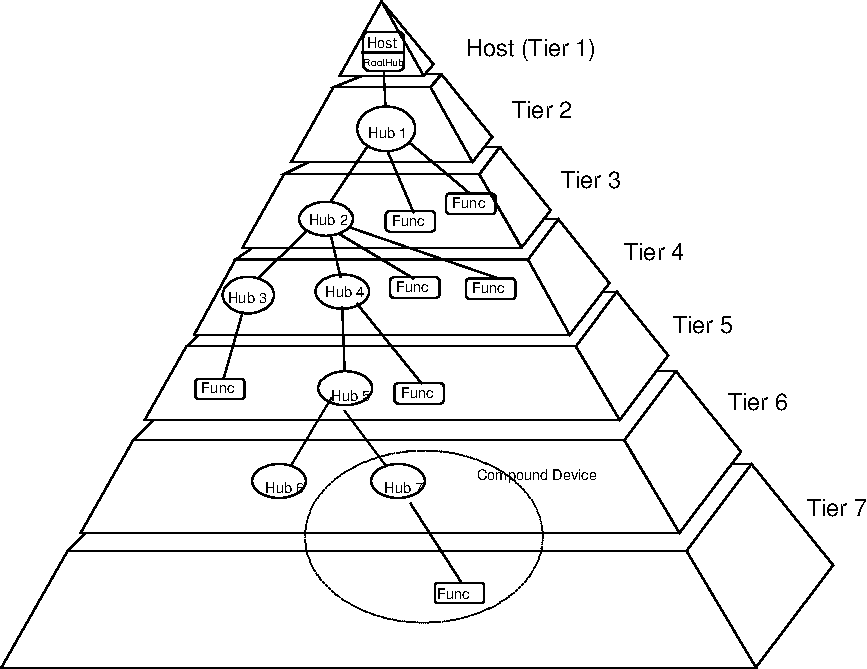
\includegraphics[width=0.75\textwidth]{img/usb_bus_topology.pdf}
\caption{Topologia do barramento USB}
\label{fig:usb_topology}
\end{figure}

A conexão de equipamentos \ac{USB} segue uma topologia de estrela em
camadas, que também pode ser entendida como uma árvore. No centro da estrela
(ou na raiz da árvore) temos obrigatoriamente o \textit{host}, que
normalmente é um computador. Por definição, o \textit{host} contém um
\textit{root hub}. Cada cabo \ac{USB} é uma conexão ponto-a-ponto que liga
um \textit{hub} da camada imediatamente acima a um dispositivo na camada
imediatamente abaixo. Um dispositivo pode ser um outro \textit{hub} ou então
uma função. Por limitações de tempo de propagação, o número máximo de
camadas é 7, incluindo a camada que contém o \textit{host}.
\cite[p.~16]{usb20}

A especificação \ac{USB} define dois tipos de conectores (conforme ilustrado
na figura \ref{fig:usb_connectors}). Um cabo \ac{USB} possui uma ponta de
cada tipo, sendo que o plugue do tipo A é conectado ao \textit{hub} da
camada acima, e o plugue do tipo B é conectado ao dispositivo da camada
abaixo. Posteriormente, foram também especificados conectores de tamanho
mais reduzido (Mini e Micro), mas os conceitos continuam os mesmos.

O protocolo de comunicação do \ac{USB} pode ser entendido como uma
arquitetura \textit{master/slave}, na qual o \textit{host} é o
\textit{master} e os dispositivos têm o papel de \textit{slave}. Só há um
\textit{host} por barramento \ac{USB}, e ele é responsável por iniciar e
gerenciar cada transação.  Como consequência, a maior parte da lógica está
centralizada no \textit{host}, simplificando bastante a implementação de
dispositivos que se conectam ao barramento \ac{USB}. \cite{usbinanutshell}

Em novembro de 2008, foi lançada a especificação do USB 3.0, que introduziu
uma quarta velocidade: \textit{super speed} (\SI{5}{\giga\bit\per\second}).
A quantidade de mudanças para suportar essa nova velocidade é grande, e foge
ao escopo deste trabalho.

% Não falei sobre:
% * Endpoints e tipos de transferências
% * *(control, interrupt, isochronous, bulk)
% * Descriptors
% * * Device Descriptor
% * * Configuration Descriptor
% * * Interface Descriptor
% * * Endpoint Descriptor
% * * String Descriptor


\section{USB HID\label{sec:usb_hid}}

Descrição do USB HID.

\section{I²C\label{sec:i2c}}

Breve descrição do protocolo \ac{I2C}.

\section{Microcontrolador ATmega8\label{sec:atmega8}}

ATmega8 é um microcontrolador de 8 bits da família AVR, fabricado pela Atmel
Corporation. Suas características principais são \cite{ATmega8}:

\begin{itemize}
\item Arquitetura Harvard, com espaços de endereçamento distintos para 
instruções e para variáveis.
\item \num{8192} bytes de memória \textit{Flash} para guardar o programa.
\item \num{512} bytes de memória \ac{EEPROM} para guardar parâmetros de configuração do
programa.
\item \num{1024} bytes de memória \ac{SRAM} para as variáveis.
\item Voltagem de operação de \SIrange{4.5}{5.5}{\volt}.
\item Clock máximo de \SI{16}{\mega\hertz}.
\item Interface de comunicação serial \ac{I2C}, com o nome de \ac{TWI}.
\end{itemize}

% TODO: completar esta seção
TODO: completar esta seção

\section{Sensor HMC5883\label{sec:sensor}}

Descrição de como o sensor funciona.


\chapter{Descrição do hardware\label{cap:hardware}}

Explicar de maneira geral as partes do circuito.

Falar sobre microcontrolador, cristal, LEDs e botões.

Inserir aqui o diagrama do circuito.

\section{Interface USB\label{sec:hardware_usb}}

Comunicação entre a USB e o microcontrolador.

Falar sobre o resistor para indiciar low speed.

\section{Interface com o sensor\label{sec:hardware_sensor}}

Problemas com I²C. ``Fonte'' 3V3 para o sensor. Level shifting para I²C.


\chapter{Descrição do software\label{cap:software}}

\section{Bootloader\label{sec:bootloader}}

\section{Comunicação I²C/TWI\label{sec:twi}}

\section{Driver V-USB\label{sec:vusb}}

Falar que implementa USB 1.1 (eu acho que é 1.1), low speed.
Falar sobre o consumo de 100mA.
Falar sobre os tipos de endpoints.
Falar sobre limitações, como por exemplo não
implementar o Suspend.

Falar aqui também sobre a implementação de um teclado. Talvez numa
subsection.

\section{Menu de configuração\label{sec:menu}}

Talvez falar sobre o teclado aqui dentro, não sei.

\section{Transformação de coordenadas\label{sec:coordenadas}}

Falar sobre: ferramentas auxiliares, teoria, resultados.

Falar sobre calibração dos cantos.

Falar sobre calibração do zero (ou deixar para falar isso depois).

\section{Mouse USB\label{sec:mouse}}

Falar sobre a implementação do mouse (que na verdade é absolute pointing
device).

Talvez aqui, talvez numa outra (sub)seção, falar sobre o fluxo da main().

\section{Outros problemas\label{sec:outros_problemas}}

\subsection{Debouncing dos botões\label{sec:debouncing}}

\subsection{Tamanho do firmware\label{sec:firmware_size}}

\subsection{Gravar configurações na EEPROM\label{sec:eeprom}}

Falar sobre gravar na EEPROM de maneira não bloqueante.

\chapter{Conclusões\label{cap:conclusoes}}

Resultados alcançados. O que deu certo. O que não deu certo.

\section{Trabalhos futuros\label{sec:trabalhos_futuros}}

Listar o que pode ser feito a partir deste projeto.


%%fakesection  Bibliografia

\bibliographystyle{abnt-num}
\bibliography{mouse_magnetometro_monografia}

% How to add \url{} to "url=" entries from Pybliographic:
% :%s/\(url\s*=\s*{\)\([^\\].*[^}]\)\(},\?\)/\1\\url{\2}\3/

%%fakesection  Anexo
\anexo

\end{document}

% vim:filetype=tex ts=4 sw=4 noet tw=76
